\section{K-means 聚类}
\label{sec:chapter11}

\subsection{聚类问题}

聚类问题属于无监督学习的范畴，与有监督学习不同，无监督学习的数据不再包含标注的标签。聚类问题就是在无标注的情况下将数据集分为若干类的问题。


\subsection{K-means 算法}

K-means 算法是解决聚类问题的一种算法，其基本思想非常简单：假设我们要将数据分为 $K$ 类，首先我们随机 $K$ 个聚类中心，然后反复执行以下步骤：
\begin{enumerate}
    \item 根据数据点到这 $K$ 个聚类中心的距离进行分类（距离哪个中心小就分为哪一类）；
    \item 将聚类中心重置为它所代表的那一类的所有点的平均位置。
\end{enumerate}

直到聚类中心不再改变，算法结束。

对于 K-means 算法，我们可以定义一个代价函数，为各数据点到它所属于的聚类中心的距离之平方和。很容易证明，1、2 两个步骤都是在减小这个代价，所以正确实现的 K-means 算法的代价应随着迭代次数增加而减小。

注意：
\begin{enumerate}
    \item 在实践中，我们可以任取 $K$ 个数据点作为聚类中心；
    \item 如果更新聚类中心时，没有数据属于某一聚类中心，则可以将该聚类中心删去（这样分类数会减少）或者置于随机位置上（保持分类数不变）；
    \item 执行一次 K-means 的结果依赖于聚类中心的选取方式，因此有可能得到一个局部最优解。所以我们可以多次执行算法，取代价最小的结果为最终结果。
\end{enumerate}


\subsection{代码实现}

\paragraph{平面点集分类}

首先看看数据集的样子：

\begin{figure}[H]
    \centering
    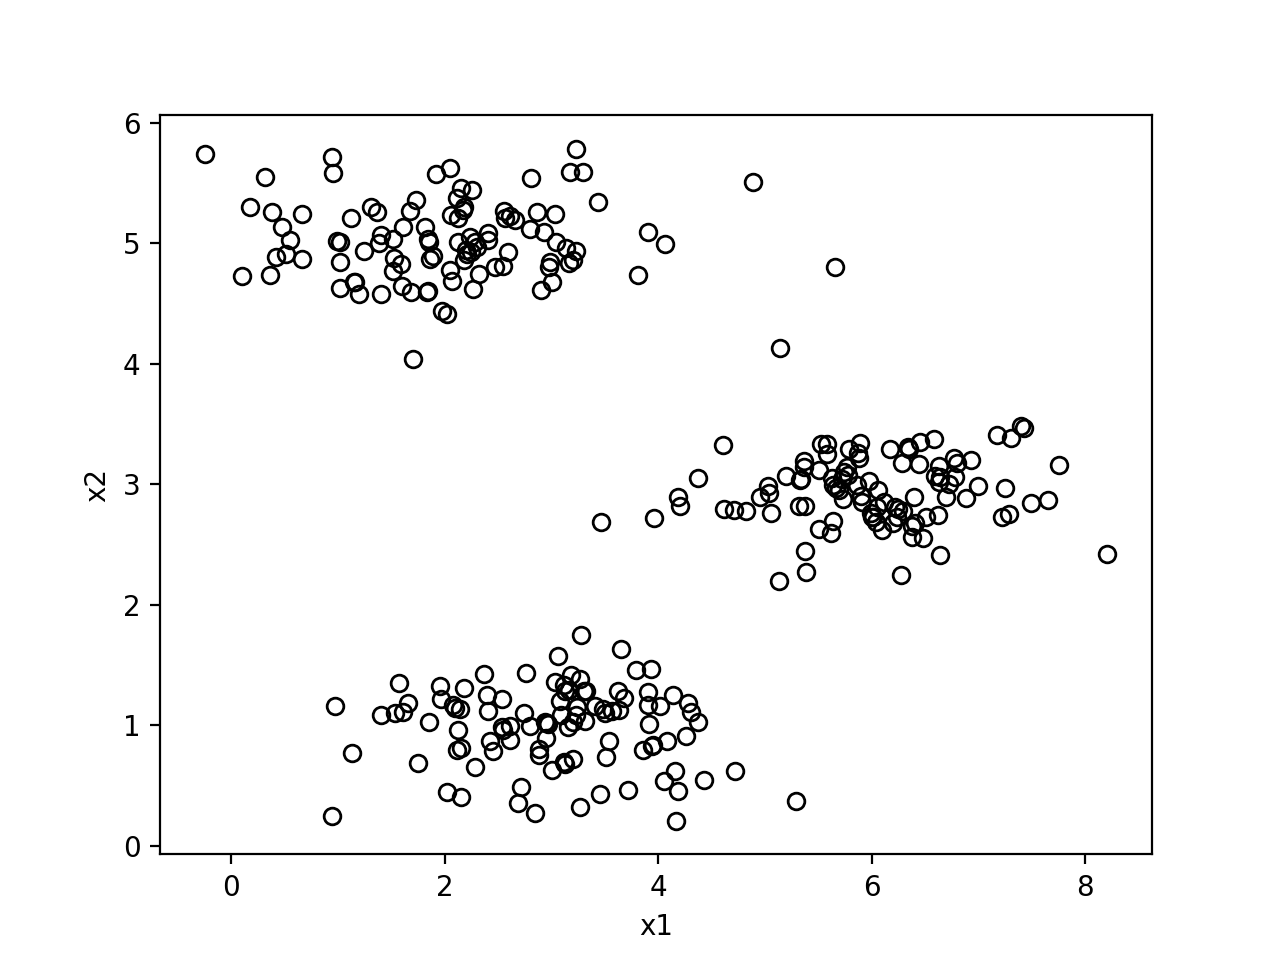
\includegraphics[width=0.5\linewidth]{figs/Chap_11_Figure_0.png}
\end{figure}

\begin{lstlisting}[language=Python]
import numpy as np
from scipy.io import loadmat
import matplotlib.pyplot as plt

X = loadmat('ex7data2.mat')['X']

def J(X, cluster, centroid):
	res = 0
	for i in range(X.shape[0]):
		res += np.dot(X[i]-centroid[cluster[i]], X[i]-centroid[cluster[i]])
	return res

def K_means(K, X, iteration=100):
	(m, n) = X.shape
	bestCluster, bestCentroid, bestJ = np.empty(m), np.empty((K, n)), np.inf
	for iter in range(iteration):
		centroid = X[np.random.randint(0, m, K)]
		cluster = np.empty(m, dtype='int')
		while True:
			ncentroid = np.zeros((K, n))
			cnt = np.zeros(K)
			for i in range(m):
				cluster[i] = np.argmin(np.sum((X[i]-centroid)**2, axis=1))
				ncentroid[cluster[i]] += X[i]
				cnt[cluster[i]] += 1
			ncentroid[cnt!=0] /= cnt[cnt!=0][:, np.newaxis]
			ncentroid[cnt==0] = X[np.random.randint(0, m, len(cnt[cnt==0]))]
			if (centroid == ncentroid).all():
				break
			centroid = ncentroid.copy()
		cost = J(X, cluster, centroid)
		if cost < bestJ:
			bestCluster, bestCentroid, bestJ = cluster.copy(), centroid.copy(), cost.copy()
	return bestCluster, bestCentroid

cl, ce = K_means(3, X, iteration=100)

ax = plt.subplot(1, 1, 1)
ax.set_xlabel('x1')
ax.set_ylabel('x2')
ax.plot(X[cl==0][:, 0], X[cl==0][:, 1], 'o', color='blue', markerfacecolor='none', alpha=0.4)
ax.plot(X[cl==1][:, 0], X[cl==1][:, 1], 'o', color='green', markerfacecolor='none', alpha=0.4)
ax.plot(X[cl==2][:, 0], X[cl==2][:, 1], 'o', color='red', markerfacecolor='none', alpha=0.4)
ax.plot(ce[0, 0], ce[0, 1], '*', color='blue', ms=10)
ax.plot(ce[1, 0], ce[1, 1], '*', color='green', ms=10)
ax.plot(ce[2, 0], ce[2, 1], '*', color='red', ms=10)
ax.plot([], [], '*', color='black', ms=10, label='cluster centroid')
ax.legend()

plt.show()
\end{lstlisting}

结果如下：

\begin{figure}[H]
    \centering
    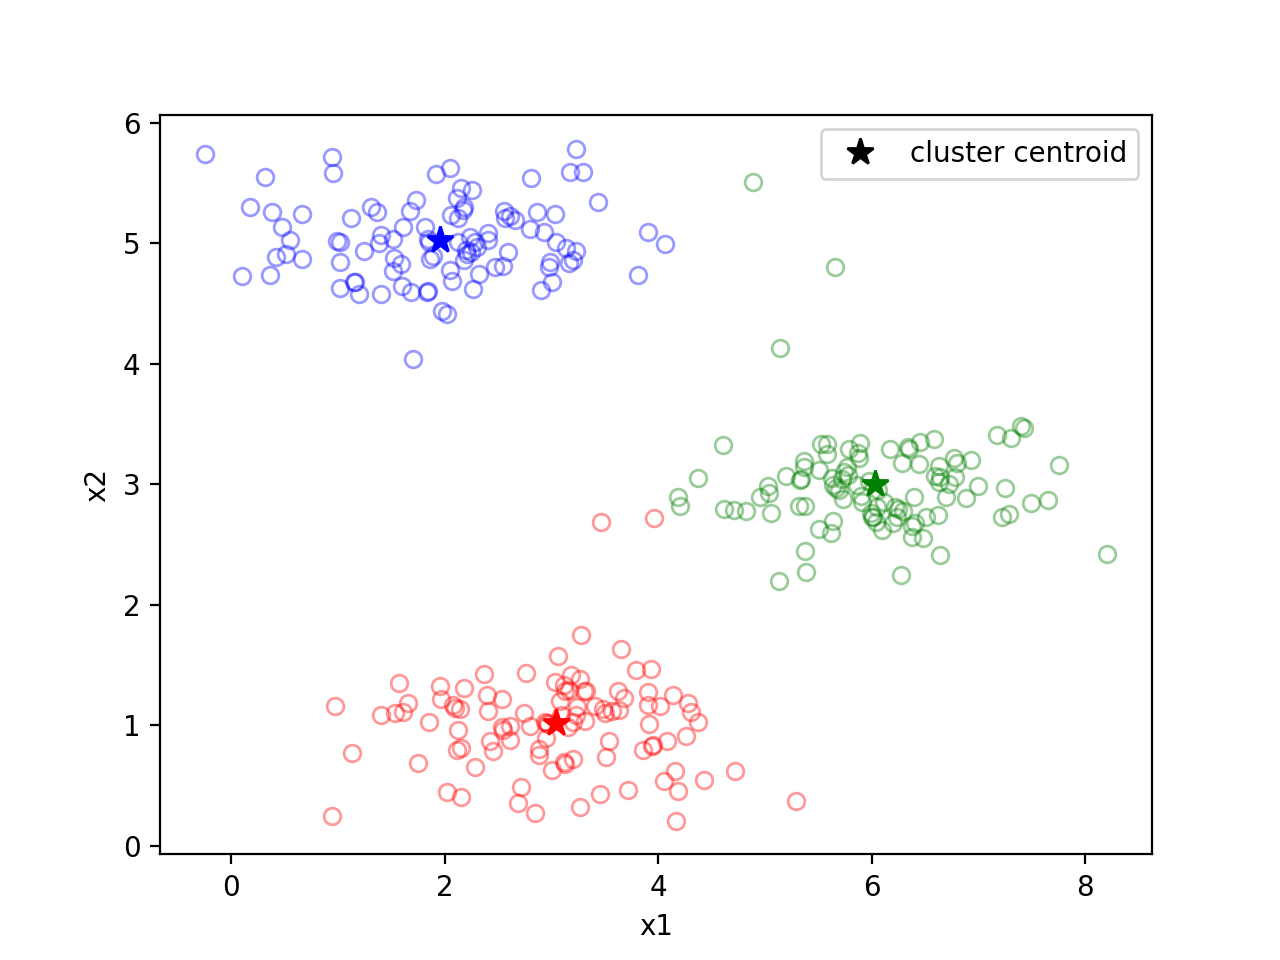
\includegraphics[width=0.5\linewidth]{figs/Chap_11_Figure_1.png}
\end{figure}


\paragraph{图像压缩}

图像是有若干像素组成的，每个像素存放 $3$ 个字节的信息代表其 $\text{RGB}$ 颜色，一张图片可能含有成百上千种颜色，如果我们只用 $16$ 种颜色表示它，那么我们只需要在对应像素位置存放一个 $4$ 位二进制数表示是第几种颜色，这样就把图像压缩到了原来的 $\frac{1}{6}$ 大小。

现在我们用 $\textbf{K-means}$ 算法去得到这 $16$ 种颜色。

我们使用的图像含有 $128\times128$ 个像素，可以处理为 $(128\times128,3)$ 的二维数组，每一行就是一个像素，包含 $3$ 个值，即 $\text{RGB}$. 这就是我们的输入数据。原图如下：

\begin{figure}[H]
    \centering
    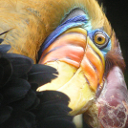
\includegraphics[width=0.3\linewidth]{figs/Chap_11_bird_small.png}
\end{figure}


\begin{lstlisting}[language=Python]
import numpy as np
from PIL import Image

def readin():
	data = np.array(Image.open('bird_small.png'))
	data = data.reshape((128*128, 3))
	return data

def J(X, cluster, centroid):
	res = 0
	for i in range(X.shape[0]):
		res += np.dot(X[i]-centroid[cluster[i]], X[i]-centroid[cluster[i]])
	return res

def K_means(K, X, iteration=100):
	(m, n) = X.shape
	bestCluster, bestCentroid, bestJ = np.empty(m), np.empty((K, n)), np.inf
	for iter in range(iteration):
		centroid = X[np.random.randint(0, m, K)]
		cluster = np.empty(m, dtype='int')
		while True:
			ncentroid = np.zeros((K, n))
			cnt = np.zeros(K)
			for i in range(m):
				cluster[i] = np.argmin(np.sum((X[i]-centroid)**2, axis=1))
				ncentroid[cluster[i]] += X[i]
				cnt[cluster[i]] += 1
			ncentroid[cnt!=0] /= cnt[cnt!=0][:, np.newaxis]
			ncentroid[cnt==0] = X[np.random.randint(0, m, len(cnt[cnt==0]))]
			if (centroid == ncentroid).all():
				break
			centroid = ncentroid.copy()
		cost = J(X, cluster, centroid)
		if cost < bestJ:
			bestCluster, bestCentroid, bestJ = cluster.copy(), centroid.copy(), cost.copy()
	return bestCluster, bestCentroid

X = readin()
cl, ce = K_means(16, X, iteration=20)

comImg = np.empty((128*128, 3), dtype='uint8')
for i in range(128*128):
	comImg[i] = np.floor(ce[cl[i]])
comImg = comImg.reshape((128, 128, 3))
im = Image.fromarray(comImg)
im.save('bird_compression.png')
\end{lstlisting}

得到的压缩结果如下：

\begin{figure}[H]
    \centering
    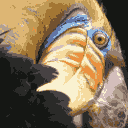
\includegraphics[width=0.3\linewidth]{figs/Chap_11_bird_compression.png}
\end{figure}
